
\PassOptionsToPackage{table}{xcolor}

\documentclass[t,aspectratio=169]{beamer}
\usepackage[backgroundTheme=LSST2017-nologos,
  footline={William O'Mullane $\bullet$ Scoil Mhuire Clontibert $\bullet$ 18$^{th}$ June 2018},
  fonts=false, colorlinks=false,
position={DM Project Manager}
]{LSST-beamer}





\author{William O'Mullane}
\institute{AURA/Rubin Observatory}
\title{LSST Data Management }
\date{  \today}


\graphicspath{ {./images/} {./ETCcharts/} }

\def\pasp{PASP}

\usepackage{pdfpages}
\usepackage{amsmath,graphicx,marvosym}
\usepackage{tikz,multirow,array,colortbl,multimedia}
\usepackage{times,layouts}
\usepackage{tikz,hyperref}
\usetikzlibrary{positioning,arrows,shapes,decorations.shapes,shapes.arrows}
\usetikzlibrary{backgrounds,calc, shadows}
\usetikzlibrary{shapes.callouts}

\usepackage{graphicx}
\usepackage{natbib}
\usepackage{longtable}

\tikzstyle{flow}=[->, >=stealth', thick, shorten >=3pt, shorten <=3pt]

\def\aaps{A\&AS}           % Astronomy and Astrophysics Suplement
\def\aap{A\&A}             % Astronomy and Astrophysics
\def\ssr{Space~Sci.~Rev.}  % Space Science Reviews
\def\apj{ApJ}              % Astrophysical Journal
\def\aj{AJ}                % Astronomical Journal
\def\mnras{MNRAS}          % Monthly Notices of the RAS
\def\araa{ARA\&A}          % Annual Review of Astron and Astrophys
\def\nat{Nature}           % Nature
\def\apjl{ApJ}             % Astrophysical Journal, Letters

\def\degr{\hbox{$^\circ$}}
\def\arcmin{\hbox{$^\prime$}}
\def\arcsec{\hbox{$^{\prime\prime}$}}
\def\fs{\hbox{$.\!\!^{\rm s}$}}
\def\fdg{\hbox{$.\!\!^\circ$}}
\def\farcm{\hbox{$.\mkern-4mu^\prime$}}
\def\farcs{\hbox{$.\!\!^{\prime\prime}$}}
\def\sun{\hbox{$\odot$}}


%\newcommand{\bfvec}[1]{\mbox{$\bf#1$}}
%\newcommand{\citell}{\citeyear}
\newcommand{\citeds}{\citeyear}
%\newcommand{\citellp}{\citeyearpar}
%\newcommand{\citedsp}{\citeyearpar}
\providecommand{\secref}[1]{Section~\ref{#1}}
\providecommand{\appref}[1]{Appendix~\ref{#1}}
\providecommand{\partref}[1]{Part~\ref{#1}}
\providecommand{\tabref}[1]{Table~\ref{#1}}
\providecommand{\figref}[1]{Figure~\ref{#1}}
\providecommand{\eqnref}[1]{Eq.~\ref{#1}}
\providecommand{\reqref}[1]{Req.~\ref{#1}}
\providecommand{\actref}[1]{AI~\ref{#1}}


\newcommand{\jira}[1]{\href{https://jira.lsstcorp.org/browse/#1}{#1}}


\title[Measuring the Galaxy ]{Measuring our galaxy and beyond}
\date{18$^{th}$ July 2018 Scoil Mhuire, Clontibret, Monaghan, Ireland}




% ----------------------


\AtBeginSection[]  % "Beamer, do the following at the start of every section"
{
\hspace*{10pt}
\begin{frame}<beamer>
\frametitle{Outline of the talk } % make a frame titled "Outline"
\tableofcontents[currentsection]  % show TOC and highlight current section
\end{frame}
}


\begin{document}

\maketitle
\frame{\frametitle{ Early background}
\begin{itemize}
\item 1982-87 High School in Fethard Co. Tipperary
\item 1984ish started with BASIC on a  Commodore (still kept horses)
\item 1987-93 MSc BSc Computer Science, University College Cork, Ireland
\item 1993 iESA Young Graduate Trainee - ESOC Germany.
\item 1994-97 Spacecraft Control Systems (C++), ESA ESOC  Germany
\item 1997-2001 Hipparcos, Integral, Planck, Gaia, Bepi-Sax  (C,Java,Oracle, HTM, HEALPix), ESA ESTEC Netherlands
\item 2012  PhD in Physics on Implementing the Gaia Astrometric Solution,  Barcelona University
\end{itemize}

YGT is still running - "about 100 YGT job offers, aimed mainly at engineers and physicists, graduates in Information Technology, Natural or Social Science and Business"\\
\url{https://www.esa.int/About_Us/Careers_at_ESA/Graduates_Young_Graduate_Trainees}
}


\frame{\frametitle{South of Spain  }
\begin{center}
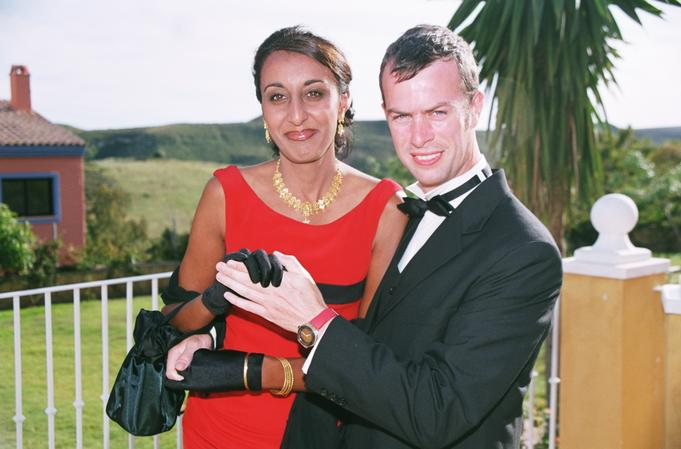
\includegraphics[width=0.9\textwidth]{rw}
\end{center}
}


\section{European Space Agency }
\frame{\frametitle{European Space Agency}
\vspace{-0.1cm}
\centering
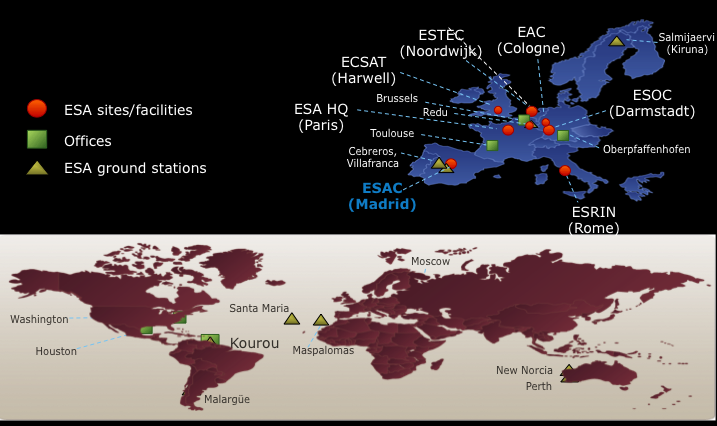
\includegraphics[width=0.9\textwidth]{esaloc}
}

\frame{\frametitle{European Spacecraft Operations Centre}
\vspace{3pt}
\begin{columns}[c]
\column{0.5\textwidth}
Late 1990s SCOSII software contractors
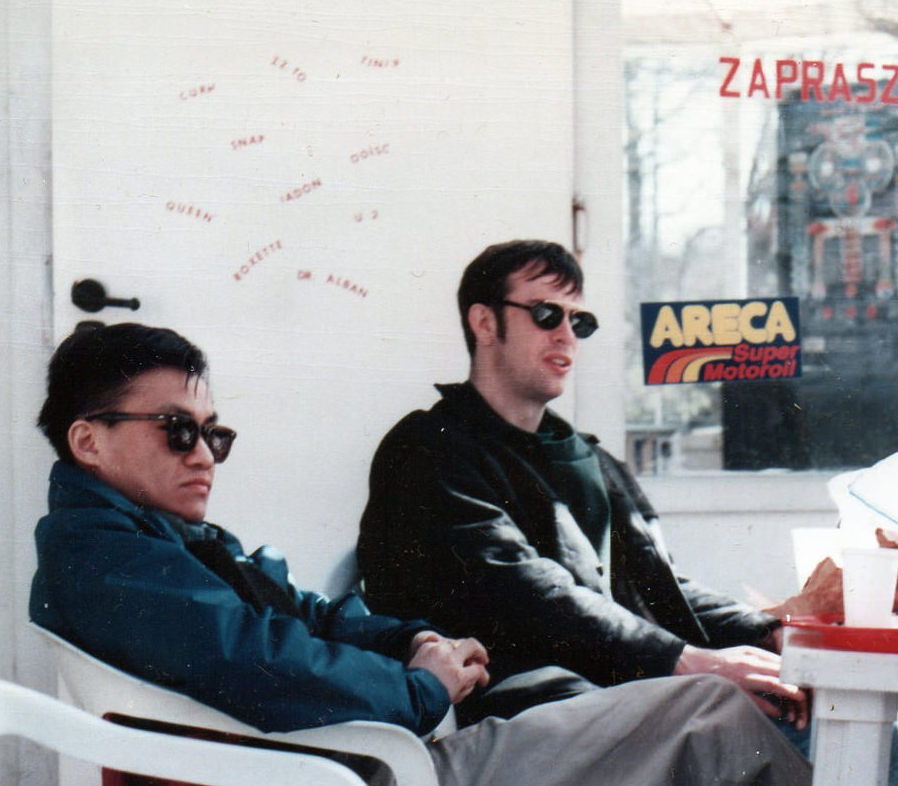
\includegraphics[width=\textwidth]{wom96}
\column{0.5\textwidth}
\begin{itemize}
\item ESOC - Located in Darmstadt, near Frankfurt, Germany.
\item Controls all ESA satellites.
\item System design/engineering, requirements management, advanced studies ..
\item  SCOSII (Satellite Control and Operations System) for ENVISAT

\end{itemize}
\end{columns}
}

\frame{\frametitle{European Space Technology Research  Centre}
\begin{columns}[c]
\column{0.5\textwidth}
 1998 Integral in ESTEC
\vspace{-1cm}
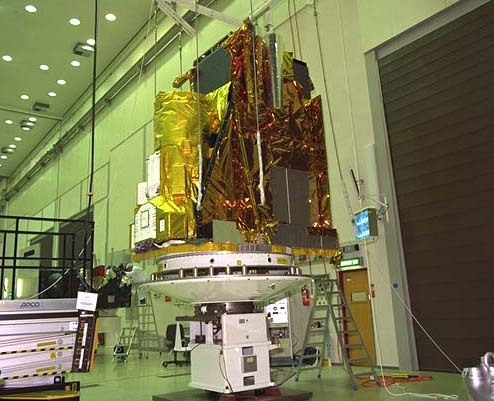
\includegraphics[width=\textwidth]{int98}\\
\column{0.5\textwidth}
\begin{itemize}
\item ESTEC - Located near Noordwijk, Netherlands.
\item Worked on Hipparcos, Integral, Planck and Gaia study phase:
\begin{itemize}
\item First ideas on Global Astrometric Solution \citep{1999BaltA...8...57O} and {\color{red} how to make a consortium}.
\item How to tesselate the celestial  sphere : HEALPix and HTM work proved popular \citep{2001misk.conf..638O}.
\end{itemize}
\end{itemize}
\end{columns}
}

\frame{\frametitle{Addition to HIP Catalogue}
1997/98 Hipparcos Java Tools - learning Astrometry
\url{http://www.cosmos.esa.int/web/hipparcos/java-tools}
\includegraphics[width=\textwidth]{hipjt}
}


\frame{\frametitle{In the USA early 2000s}
\vspace{5pt}
\begin{columns}[c]
\column{0.6\textwidth}
Entering the new millennium ..  \\
\vspace{4pt}
Quality tools for GSC2 (Java) $\rightarrow$\\
\vspace{8pt}
CasJobs (C\#)\citep{2004ASPC..314..372O}
\includegraphics[width=\textwidth]{casjobs}
\column{0.4\textwidth}
\includegraphics[width=\textwidth]{sshtm}
\vspace{-1cm}
\includegraphics[width=\textwidth]{showsky}
\end{columns}
}


\frame{\frametitle{European Space Astronomy Centre}
\begin{columns}[c]
\column{0.4\textwidth}
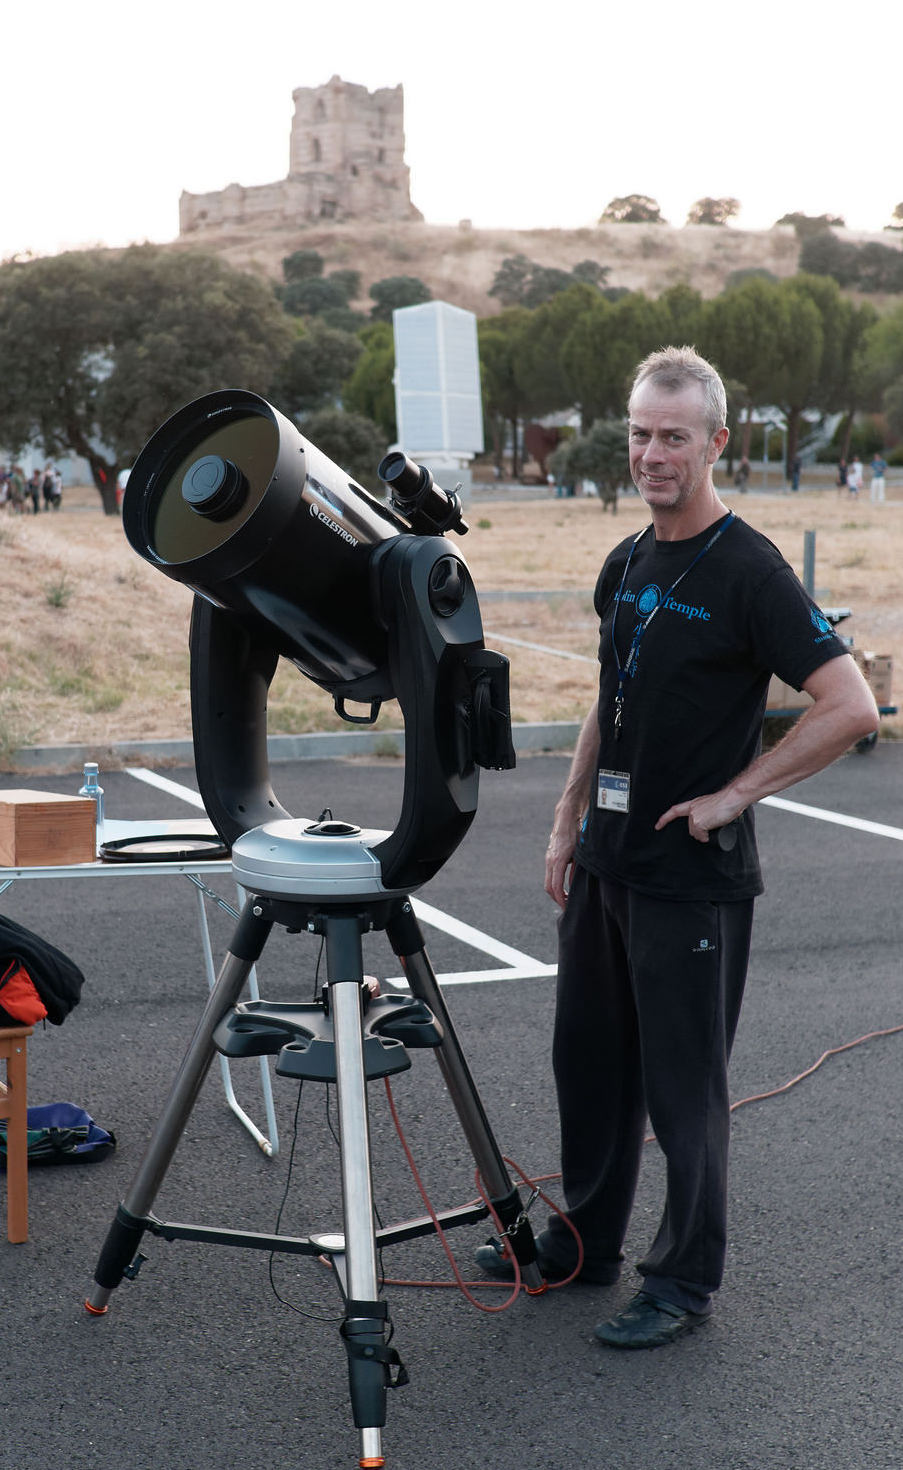
\includegraphics[width=\textwidth]{wom2016}\\
\column{0.6\textwidth}
\vspace{-1cm}
 \\
From 2005 to 2017\\
\begin{itemize}
\item ESAC Located near Madrid, Spain.
\item Home of the Science Operations Department of the Eurpoean Space Agency
\item Surprising number of Irish people ..
\item This picture from a public stargaxing night - $\sim$400 visitors came

\end{itemize}
\end{columns}
}




\frame{
\frametitle{Operations and Archiving}
\begin{center}
\setbeamercovered{invisible}
\vspace{-1.5cm} \includegraphics[width=0.7\textwidth] {images/esasky}
\vspace {-8cm}
{\color{yellow} \large
%\rowcolors{1}{blue!20}{blue!20}
\begin{tabular}{p{\textwidth}}
\onslide<2->{\hspace {2cm}\bf  Lots of  missions flying and finished, all  data  in ESAC.}\\
\\
\\
\\
\onslide<2-> {\hspace{2cm} \bf  ESA Sky - \url{http://sky.esa.int//} }\\

\end{tabular}
}

\end{center}
}



\section {Gaia and LSST }

\frame{\frametitle{ A little about myself}
	\vspace{-3pt}
\begin{itemize}
\item 1985ish started with BASIC on a  Commodore
\item 1993 MSc BSc Computer Science, University College Cork, Ireland
\item 1993 - 1997 Spacecraft Control Systems (C++), ESA ESOC  Germany
\item 1997 - 2001 Hipparcos, Integral, Planck, Gaia, Bepi-Sax  (C,Java,Oracle, HTM, HEALPix), ESA ESTEC Netherlands
\item 2001-2003 Commercial programming - some Astronomy (Java)
\item 2003-2005 The Johns Hopkins, SDSS and National Virtual Observatory (C,C\#,Java,Sqlserver)
\item 2005-2014 Gaia Astrometric Solution and Science Operations (Java, Oracle, Intersystems Cache)
\item 2012  PhD on Implementing the Gaia Astrometric Solution,  Barcelona University
\item 2014-2017 ESA SCI-OD division head - all science ground segments in development
\item 2017- LSST Data Management Project Manager (Python,C++), Deputy Project Manager for Software (control systems and IT)

\end{itemize}
}


\frame { \frametitle{ LSST:uniform sky survey }
\begin{columns}
\column{0.45\textwidth}
\vspace {-0.3cm}
 \\
An optical/near-IR survey of half the sky in ugrizy bands to r~27.5 (36 nJy) based on 825 visits over  a 10-year period: {\em deep wide fast}.
%It’s about 5,000 sq. deg. per night, *twice*, on
%average. That is, about 1,000 visits per night on average. You return to
%the same position on the sky in about 3-4 nights (in any band). Btw, it’s
%a nice coincidence worth remembering that the total exposure time per
%position over 10 years (in all bands) is equal to about one observing night.
\begin{itemize}
\item 90\% of time  spent on  uniform survey: every 3-4 nights, the whole observable sky scanned twice per night
\item	~100 PB of data: about a billion 16 Mpix images, enabling measurements\\ {\color{cyan} for 40 billion objects! }
\end{itemize}
{\tiny see also \url{http://www.lsst.org} and \cite{2008arXiv0805.2366I}-arXiv:0805.2366}

\column{0.55\textwidth}
	 \includegraphics[width=0.9\textwidth]{images/coverage}\\
\vspace {-5pt}
{\bf 10-year simulation of LSST survey: number of visits in u,g,r band (Aitoff projection of eq. coordinates) }\\
\end{columns}

}
\frame { \frametitle{ LSST Camera }
\begin{columns}
\column{0.6\textwidth}
 \includegraphics[width=1.0\textwidth]{images/camera}
\column{0.4\textwidth}
 \\
\vspace {-3cm}
{\large \bf The largest astronomical camera:}
\begin {itemize}
\item 2800 kg
\item 3.2 Gpix
\end {itemize}
\end{columns}
}

\frame { \frametitle{ Site as imagined and in March 2019 }
\begin{columns}
\begin{column}{0.5\textwidth}
\vspace {7cm}
	\includegraphics[width=0.95\textwidth,trim=0cm 10cm 0 10cm,clip]{images/cerroRender}
\end{column}
\begin{column}{0.5\textwidth}
\\
	\includegraphics[width=0.95\textwidth,trim=0cm 0cm 5cm 0cm,clip]{images/cerroMar2019}
\end{column}
\end{columns}

}

\frame {\frametitle{  DM build and deploy - already challenging }
	\vspace{-1cm}
	\begin{columns}
		\column{0.4\textwidth}
		\begin{center}
			      \includegraphics[width=1.0\textwidth]{images/DMSDeployment}\\
		      \end{center}
		      \column{0.6\textwidth}
		       \\
		       \vspace{1cm}
		       DM must build everything to get LSST products (see \url{http://ls.st/dpdd})  to the users.
		       \begin{itemize}
			       \item large data sets (20TB/night)
			       \item complex analysis
			       \item aiming for small systematics
			       \item Science Alerts in under 2 minutes .. (aiming for 1 minute)
		       \end{itemize}
		       About $1\over{2}$  million lines of code (C++/python) all open source on github\\
		       \vspace{25pt}
		       {\tiny \bf diagram K.T. Lim}
	       \end{columns}
       }




\frame {\frametitle{  Data Backbone}
\begin{columns}
\column{0.45\textwidth}
      \includegraphics[width=1.0\textwidth]{images/DataBackbone}\\
\column{0.55\textwidth}
 \\
 One small box on the previous slide was Data Backbone.\\ That hides several things \\
 \begin{itemize}
	 \item Qserv - the LSST end user database
 \begin{itemize}
	 \item{\color{red} Custom Massive Parallel Processing (MPP) }
	 \item allow queries on $\approx 20$ Petabytes of tabular data
	\item $4 \times 10^{10}$ objects, $4 \times 10^{13}$ sources (observations)
 \end{itemize}
\item All the networks : we now have fiber to the mountain and from La Serena to NCSA (two routes)
 \end{itemize}
\vspace{25pt}
{\tiny \bf diagram K.T. Lim}
\end{columns}
}


\frame{\frametitle{Rubin Observatory Catalog 2035 }
Astronomy catalogs tend to be highly structured, tabular, somewhat predictable access.

\begin{columns}
\begin{column}{0.45\textwidth}

\begin{itemize}
\item Data, by DR11:
\begin{itemize}
\item  ~60T rows (mostly ForcedSource)
\item  ~10PB (mostly Source + ForcedSource + Object extra)
\end{itemize}
\item  Breakdown of most significant tables (rows x cols, storage):
\begin{itemize}
\item  Object: ~47B x 330, ~100TB
\item  Object extra: ~1.5T x 7,600, ~1.2PB
\item  Source: ~9T x 50, ~5PB
\item  ForcedSource: ~50T x 6, ~2PB
\end{itemize}
\end{itemize}
\end{column}
\begin{column}{0.55\textwidth}
\begin{itemize}
\item Get an object or data for small area - <10 sec
\item Scan through billions of objects - $\approx$ 1 hour
\item Deeper analysis (Object\_*) - $\approx$ 8 hours
\item Analysis of objects close to other objects -  $\approx$ 1 hour, even if full-sky
\item Analysis that requires special grouping - $\approx$ 1 hour, even if full sky
\item Source, ForcedSource scans - $\approx$ 12 hours
\item Cross match \& anti-cross match with external catalogs - $\approx$ 1 hour
\end{itemize}
\end{column}
\end{columns}
}


\frame{\frametitle{Qserv \tiny(slides from Fritz Muller) }

\begin{columns}
\begin{column}{0.6\textwidth}
\begin{itemize}
\item Shared-nothing MPP RDBMS (SQL, throughput, horizontal scaling)
\item  Spherical partitioning with overlap (near-neighbor self-joins)
\item  Shared scans (concurrent query load)
\item  Replicated data (resiliency)
\item  Fixed-purpose, dedicated hardware (cost, predictability)
\end{itemize}
\end{column}
\begin{column}{0.4\textwidth}

\includegraphics[width=0.90\textwidth]{images/spher}
	 Tesselation see  \cite{2001misk.conf..638O}
\end{column}
\end{columns}

Design optimized for use case + hardware efficiency \citeds{LDM-135}

Built on project at SLAC, leverage existing tech within Stanford (MariaDB, MySQL Proxy,
XRootD, Google protobuf, Flask)


100\% open source  \url{https://github.com/LSST/Qserv}
}

\frame{\frametitle{Shared Nothing Massively Parallel Processing }

\begin{columns}
\begin{column}{0.45\textwidth}

\includegraphics[width=1.1\textwidth]{images/distribute-combine}\\
		Recent scale tests: \url{https://dmtr-071.lsst.io}\\
		Perf and BigQuery: \citeds{Document-31100}
\end{column}
\begin{column}{0.5\textwidth}

\begin{itemize}
\item Ultimate target platform ~300 nodes in 2 international data-centers
\item	Development cluster (CC-IN2P3):
\begin{itemize}
\item  400 cores, 800 GB memory, 500 TB storage
\item  ~100 TB synthetic dataset on 2 x 25 nodes
\end{itemize}
\item Prototype Data Access Center (NCSA):
\begin{itemize}
	\item  500 cores, 4 TB memory, 700 TB storage
	\item  ~100 TB science dataset (SDSS Stripe 82 +
		WISE) on 30 nodes
	\item  + HSC reprocessing + GAIA DR2 coming up
\end{itemize}
\end{itemize}
\end{column}
\end{columns}
}




\frame {
  \frametitle{ Inevitably we must document ..  }

\begin{columns}
	\column{0.5\textwidth}
\begin{center}
   \includegraphics[width=0.9\textwidth,trim=0cm 0cm 0cm 0cm]{images/fops}\\
\end{center}
	\column{0.5\textwidth}
 \\
\vspace{1cm}
Gaia Flight Operations Procedures (FOP) paper copy in case the computers fail - could be useful!
\begin{center}
\vspace{5pt}
{\color{red} But we should avoid {\em write only} documents.}
\end{center}
\end{columns}
}




\frame{\frametitle{Guidelines,  tools,  conventions }
\begin{itemize}
    \item {\color{green} Its great having extensive guidelines - it was also something super on Gaia}
   \item \url{developer.lsst.io} is a full developer guide - everything from git commit messages to style guides for Python and C+.
   \item \url{pipelines.lsst.io} documents the main software release(s)
	\begin{itemize}
	\item worst of both worlds - it is a monolithic release  - but made up of > 120 git repos
	\item Still using \emph{in house} tools like EUPS \url{https://github.com/RobertLuptonTheGood/eups}
	\item moving toward conda-forge
	\item {\color{green} All open source (GPL) on github.com}
	\end{itemize}
\item  Language (spoken/written) and conventions are also super important
    \begin{itemize}
	    \item Single language projects  (like US or UK) fall more easily in the trap of \emph{believing} they speak  about the same topics because they speak language X.
	    \item {\color{blue} - on RubinObs we lack something foundational like \citeds{LL:BAS-003}}
    \end{itemize}

\end{itemize}
}


\frame {\frametitle{SDSS image }
	\begin{columns}
		\column{0.45\textwidth}
	      \includegraphics[width=1.0\textwidth]{images/SDSScosmos}\\
		      \column{0.55\textwidth}
		      \\
		       \vspace{1cm}
	       Nice colors \cite{2004PASP..116..133L}\\
	       $\approx  3.5 \arcmin$\\
		       \vspace{20mm}
	       {\tiny \bf{Image  Robert Lupton}}
	       \end{columns}
}
\frame {\frametitle{Hyper Suprime Cam (HSC) on Subaru }
\begin{columns}
      \column{0.45\textwidth}
		       \vspace{-20pt}
	      \includegraphics[width=1.0\textwidth]{images/HSCcosmos}\\
      \column{0.55\textwidth}
		       \\
		       HSC image (COSMOS) from g,r(1.5 hrs) ,i(3 hrs) PSF matched co-add ($\approx 27.5$)\\
		       Challenges:

\begin{itemize}
\item Unknown statistical distributions,   Truncated, censored and missing data, Unreliable quantities (e.g. unknown systematics and random errors)
\item PSF - short exposure - atmosphere dominated ?

\begin{itemize}
\item cosmic shear signal from weak lensing
\end{itemize}
\item Photometry  challenging - will Gaia help ..
\item Everything is blended!!
\end{itemize}
		{\tiny       Processed with  {\em LSST Stack} \url{https://pipelines.lsst.io/}\\
	        \bf{Image HSC collaboration,  Robert Lupton}}
\end{columns}
       }



\frame{\frametitle{Catalog extraction }
\begin{columns}
      \column{0.45\textwidth}
		       \vspace{-20pt}
	      \includegraphics[width=1.0\textwidth]{images/square/jupyterlab_nb}\\
      \column{0.55\textwidth}

\begin{itemize}
\item Identifying sources and disentangling them becomes more difficult as we have deeper images.
\item Left our typical Jupyter setup runs

\begin{itemize}
\item  Insrtrument signature removeval
\item  calibration
\item  source extraction
\item  overlay extracted information on cleaned image
\end{itemize}
\end{itemize}
\end{columns}
}



\section {Launch }


\frame{
\frametitle{To Kourou}
\begin{center}
\includegraphics[width=0.9\textwidth,trim=0 0 0 10pt,clip]{gaiaim/soyuz}\\
\end{center}
}

\frame{ \frametitle{Lots of interesting signs .. }
\includegraphics[width=0.55\textwidth]{gaiaim/sign}
\hfill
\includegraphics[width=0.4\textwidth]{gaiaim/sign2}
}

\frame{ \frametitle{Up close }
\begin{columns}
\column{0.4\textwidth}
\includegraphics[width=\textwidth]{gaiaim/fregat}

\column{0.6\textwidth}

\vspace{-9cm}
Dec 18th saw (touched) our Fregat.\\
Meanwhile a full dress rehearsal  ongoing.\\
Later road closed for  Ariane movement\\
\includegraphics[width=0.6\textwidth]{gaiaim/ariane}\\
\end{columns}
}

\frame{ \frametitle{Countdown.. }
\vspace{-10pt}
\begin{center}
Dec 18th 17:12 (20:12 UTC) the count down started.
In Jupiter control room
\includegraphics[width=0.9\textwidth]{gaiaim/womcsg}\\
\end{center}
}

\frame{ \frametitle{Flawless lift off 19/12 06:12am}
\vspace{-10pt}
\begin{center}
\includegraphics[width=0.7\textwidth,trim=0 0 0 0pt]{gaiaim/lo}\\
\vspace{-30pt}
{\tiny Photo: R. Gill}\\
\vspace{+5pt}
Shunshiled very flat - Gaia magnitude 20.5 (expected 19) at L2.
\end{center}
}


\frame{\frametitle{ Video clips }
\begin{itemize}
\item Gaia Launch \url{https://youtu.be/xDmQvJVJg8Y?t=87}

\item Gaia Data Release 2 \url{https://youtu.be/KULtrwVSq6g?t=10}

\item Cerro Pachon LSST \url{https://gallery.lsst.org/bp/\#/folder/2689925/64565141}

\end{itemize}
}


\section{Astrometry}
\frame {\frametitle{ Astrometric Solution}
Just one part of the Gaia processing !\\
From the Hipparcos catalogue
\cite[Volume 3 Chapter 23]{hip:catalogue}.

\begin{block}{Minimisation problem for astrometry}
\begin{equation}
	 ^{min}_{\bfvec{a},\bfvec{n}} \| \bfvec{g^{obs}} - \bfvec{g^{calc}}(\bfvec{a},\bfvec{n})\|_{M}
	\label{eq:generalobs}
\end{equation}
\end{block}
\begin{itemize}%[<+->]
\item $\bfvec{a}$  is the vector of unknowns describing a star's barycentric motion
represented by the measurement vector $\bfvec{g_{k}} = (G_{k},H_{k})^{\prime}$
and associated statistics.
\item $\bfvec{g^{obs}}$ represents the vector of all measurements
\item  $\bfvec{g^{calc}}$ represents the vector of detector
coordinates calculated from the astrometric parameters.
\item $\bfvec{n}$ is a vector
of nuisance parameters - required for realistic modeling (e.g. attitude, instrument calibration)

\item   $M$ metric defined by the statistics
of the data, (error weighting)

\end{itemize}
The complete new formulation for Gaia is in \citep{2012A&A...538A..78L}.
}


\frame {\frametitle{ Basic Gaia Problem }
%\vspace{-10pt}
Put more simply the data reduction must:\\
{\em
find the astrometric parameters (catalogue) best
predicting the ($10^{12}$) focal plane observations of the sources.
\citep{2011ExA....31..215O}
}
\begin{center}
\includegraphics[scale=0.6, clip=true,trim=1cm 0cm 0 1.5cm ]{gaiaim/predict}
\end{center}
}

\frame {\frametitle{ Look at one block: Source modeling }
%\vspace{-15pt}
The mapping or modeling  of
the observables
 $\bfvec{g}$ is done by three successive transformations:
 \begin{enumerate}%[<+->]
\item from astrometric parameters to the celestial directions of a star at the
instant of observation, using an astrometric model {\color{blue}\bf S}

\item from celestial  to instrument frame directions using an attitude
model {\color{blue}\bf A}
\item and finally from instrument directions to detector coordinates using an
instrument model {\color{blue}\bf C}
 \end{enumerate}
\vspace{-25pt}
\begin{center}
\includegraphics[scale=0.38,clip=true,trim=1cm 0cm 12cm 0 ]{gaiaim/atttoon}
\includegraphics[scale=0.38,clip=true,trim=3cm 0cm 6cm 0 ]{gaiaim/pixcoord}
\end{center}
}



\frame {\frametitle{ Source Update }
\setbeamercovered{invisible}
%\vspace{-14pt}
We fit the model to the observations:
\begin{block}{ Least squares for source update}
\begin{equation}\label{eq:lsobsmatrix}
\bfvec{Ax} \sim \bfvec{b} \pm \bfvec{\sigma}
\end{equation}
\begin{equation}
 \text{where~} \bfvec{b}_{i} = \bfvec{y}_{i}- f_{i}(\bfvec{a,q})
 \label{eq:f}
\end{equation}
\end{block}
Here $\bfvec{y}_{i}$ are the observed field angles  $f_{i}$ is a function to calculates field angles
from the current model.\\
\pause
In java (SourceUpdateCalculatorWrapper):
\includegraphics[width=\textwidth]{gaiaim/srcup}\\
\citep{2011ExA....31..215O}
}


\frame{\frametitle{Its all team work on big projects }
\centering
\includegraphics[width=\textwidth]{gaiaim/agis17}\\
}


\frame {
  \frametitle{ The END }
\vspace{-0.3cm}
\begin{center}
 \includegraphics[width=0.4\textwidth]{images/SDSScosmos}
\hfill
 \includegraphics[width=0.4\textwidth]{images/HSCcosmos}\\
\vspace{-3.2cm}\hspace{0.7cm} \huge{\color{red} Questions?}\\
\vspace{+2.2cm}
\normalsize
{$\sim  3.5 \arcmin$ SDSS image   \hfill  HSC image (COSMOS)   \\\hfill \tiny g,r(1.5 hrs) ,i(3 hrs) PSF matched co-add ($\approx 27.5$)\\}

\vspace{-5pt}
{\tiny \url{http://www.lsst.org}} {\tiny \url{http://community.lsst.org}} \hfill
{\tiny Images:Lupton and HSC colaboration see also \cite{2004PASP..116..133L}}
\end{center}

}


\frame[allowframebreaks]{\frametitle{ Acronyms }
\vspace{10pt}
\tiny
\addtocounter{table}{-1}
\begin{longtable}{|l|p{0.8\textwidth}|}\hline
\textbf{Acronym} & \textbf{Description}  \\\hline

AURA&Association of Universities for Research in Astronomy \\\hline
C&Specific programming language (also called ANSI-C) \\\hline
DM&Data Management \\\hline
ESA&European Space Agency \\\hline
ESAC&European Space Astronomy Centre (VilSpa) \\\hline
ESOC&European Space Operations Centre (ESA) \\\hline
ESTEC&European Space research and TEchnology Centre (ESA) \\\hline
HEALPix&Hierarchical Equal-Area iso-Latitude Pixelisation \\\hline
HTM&Hierarchical Triangular Mesh \\\hline
LSST&Large Synoptic Survey Telescope \\\hline
PhD&Doctorate in Philosophy \\\hline
SDSS&Sloan Digital Sky Survey \\\hline
TEC&Thermo-Electric Cooler \\\hline
USA&United States of America \\\hline
arcmin&arcminute, minute of arc (unit of angle) \\\hline
arcsec&arcsecond, second of arc (unit of angle) \\\hline
\end{longtable}

}
\frame{\frametitle{ References }
\tiny
\bibliographystyle{gaia_aa}
\bibliography{lsst,gaia_livelink_valid,books,refs_ads}
\normalsize

}
\end{document}
